% お使いの環境に合わせて以下3行のdocumentclassをお選びください。
\documentclass[twocolumn]{jarticle} % pLaTeX
%\documentclass[uplatex,twocolumn]{jsarticle}  % upLaTeX
%\documentclass[xelatex,twocolumn,ja=standard,enablefam=true]{bxjsarticle} % XeLaTeX

\usepackage{rsj2024j}
\usepackage[dvipdfmx]{graphicx}
\usepackage{url}
\usepackage{tikz}

\begin{document}
\title{2D-LiDARとYOLOv10を用いた人追従システムの開発}
\author{〇金澤 祐典(金沢工業大学)\ \ 出村\ 公成(金沢工業大学)}
\abstract{In this study, a human tracking system using 2D-LiDAR and YOLOv10 will be developed and the system will be evaluated using actual equipment in a miscellaneous environment. Ankle-level 2D-LiDAR data will be converted to overhead images, and a data set will be created using 100,000 overhead images. The created dataset and YOLOv10 will be used for deep learning; YOLOv10 is the latest real-time object detection model released in May 2024. A kachaka from Preferred Robotics, Inc. will be used for the robot platform and a UTM30-LX from Hokuyo Electric Co. will be used for 2D-LiDAR. }
\setlength{\baselineskip}{4.4mm}	% 行間の設定
\maketitle
\thispagestyle{empty}
\pagestyle{empty}



\section{はじめに}
現代社会において, 自律型技術の進化と共に, 人々の安全確保や効率的な作業プロセスの追求が重要視されている.近年では, 様々な産業や領域で人追従技術への需要が高まっている.この需要の背景には, 自動化と効率性の追求や, 安全とセキュリティの重要性, 高齢化社会と医療分野の変化, 観光業界のニーズなど, 多岐にわたる要因が存在する.

製造業や物流分野では, 自動化が加速し, 作業プロセスの効率化と品質の向上が求められている. 高齢化社会においては, 介護や医療分野での需要が増えている. 観光業界でも, 来場者の案内や体験の向上のために, 人追従技術を活用する取り組みが進んでいる. 本研究では, 屋内環境における2D-LiDARとYOLOv10\cite{yolov10}を用いた人追従システムを開発する.



\section{従来研究}
2D-LiDARを用いた人追従に関する従来研究では, 背景減算を用いて人の脚部を検出する手法\cite{mahmudul2020}や, FCNによる脚部検出の手法\cite{angel2019}がある. これらの手法では, 脚部検出はできているが, 周囲の環境に影響されやすく, 雑多な環境下での人追従は不安定であることが今後の課題として挙げられる.



\section{提案手法}
\subsection{概要}
本研究が提案する手法は, YOLOv10の物体検出モデルにより, 人の脚部を検出し, 目標座標へロボット台車を制御する人追従システムである. ソフトウェアの開発環境はUbuntu22.04でRobot Operating System 2(以下ROS2)を使用した. 

人の脚部検出では, 前処理として2D-LiDARから取得した距離データを図\ref{fig:laser_img}のような俯瞰画像へ変換する. 変換した画像をYOLOv10の物体検出モデルで学習し, 学習した重みと画像を用いて人の脚部を検出する. システム起動時は最も近い脚部を検出する. 追従中は, 1つ前のフレームにおける追従対象者の座標を円型の範囲で囲み, 範囲内に脚部が検出できた場合に追従する. ロボット台車の制御では, 目標座標までの角度の偏差と距離の偏差の2つを収束させるPD制御を実装する. 目標座標は, 人の脚部を検出したときのBounding Boxの中心座標を人の座標とし, 中心座標の後方に生成した座標を目標座標としている.

\begin{figure}[ht]
  \centering
  \large
  % eps 画像を貼る場合は includegraphics をお使いください。
  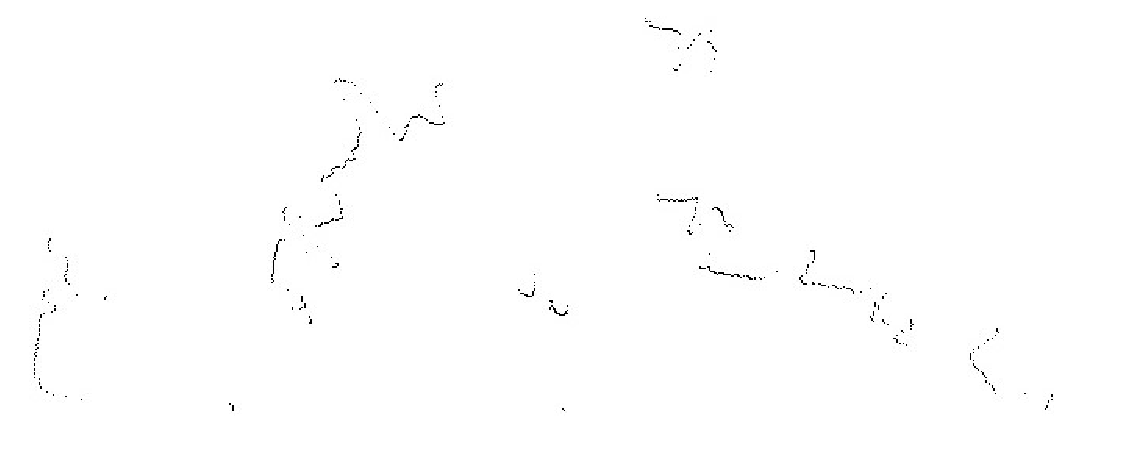
\includegraphics[width=45mm]{figure/laser_img_232.eps}
  \caption{俯瞰画像の例}
  \label{fig:laser_img}
\end{figure}

\begin{figure}[ht]
  \centering
  \large
  % eps 画像を貼る場合は includegraphics をお使いください。
  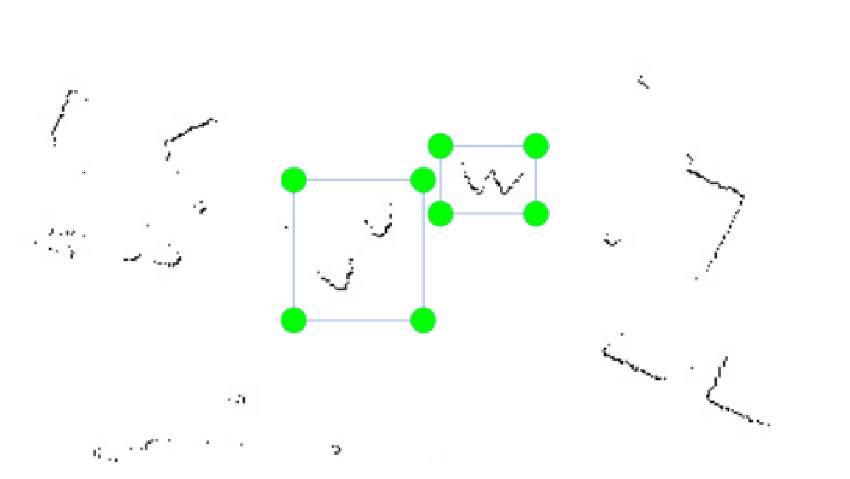
\includegraphics[width=45mm]{figure/ex-data-sets.eps}
  \caption{データセットの例}
  \label{fig:dataset}
\end{figure}

\begin{figure}[ht]
  \begin{minipage}[b]{0.45\linewidth}
    \centering
    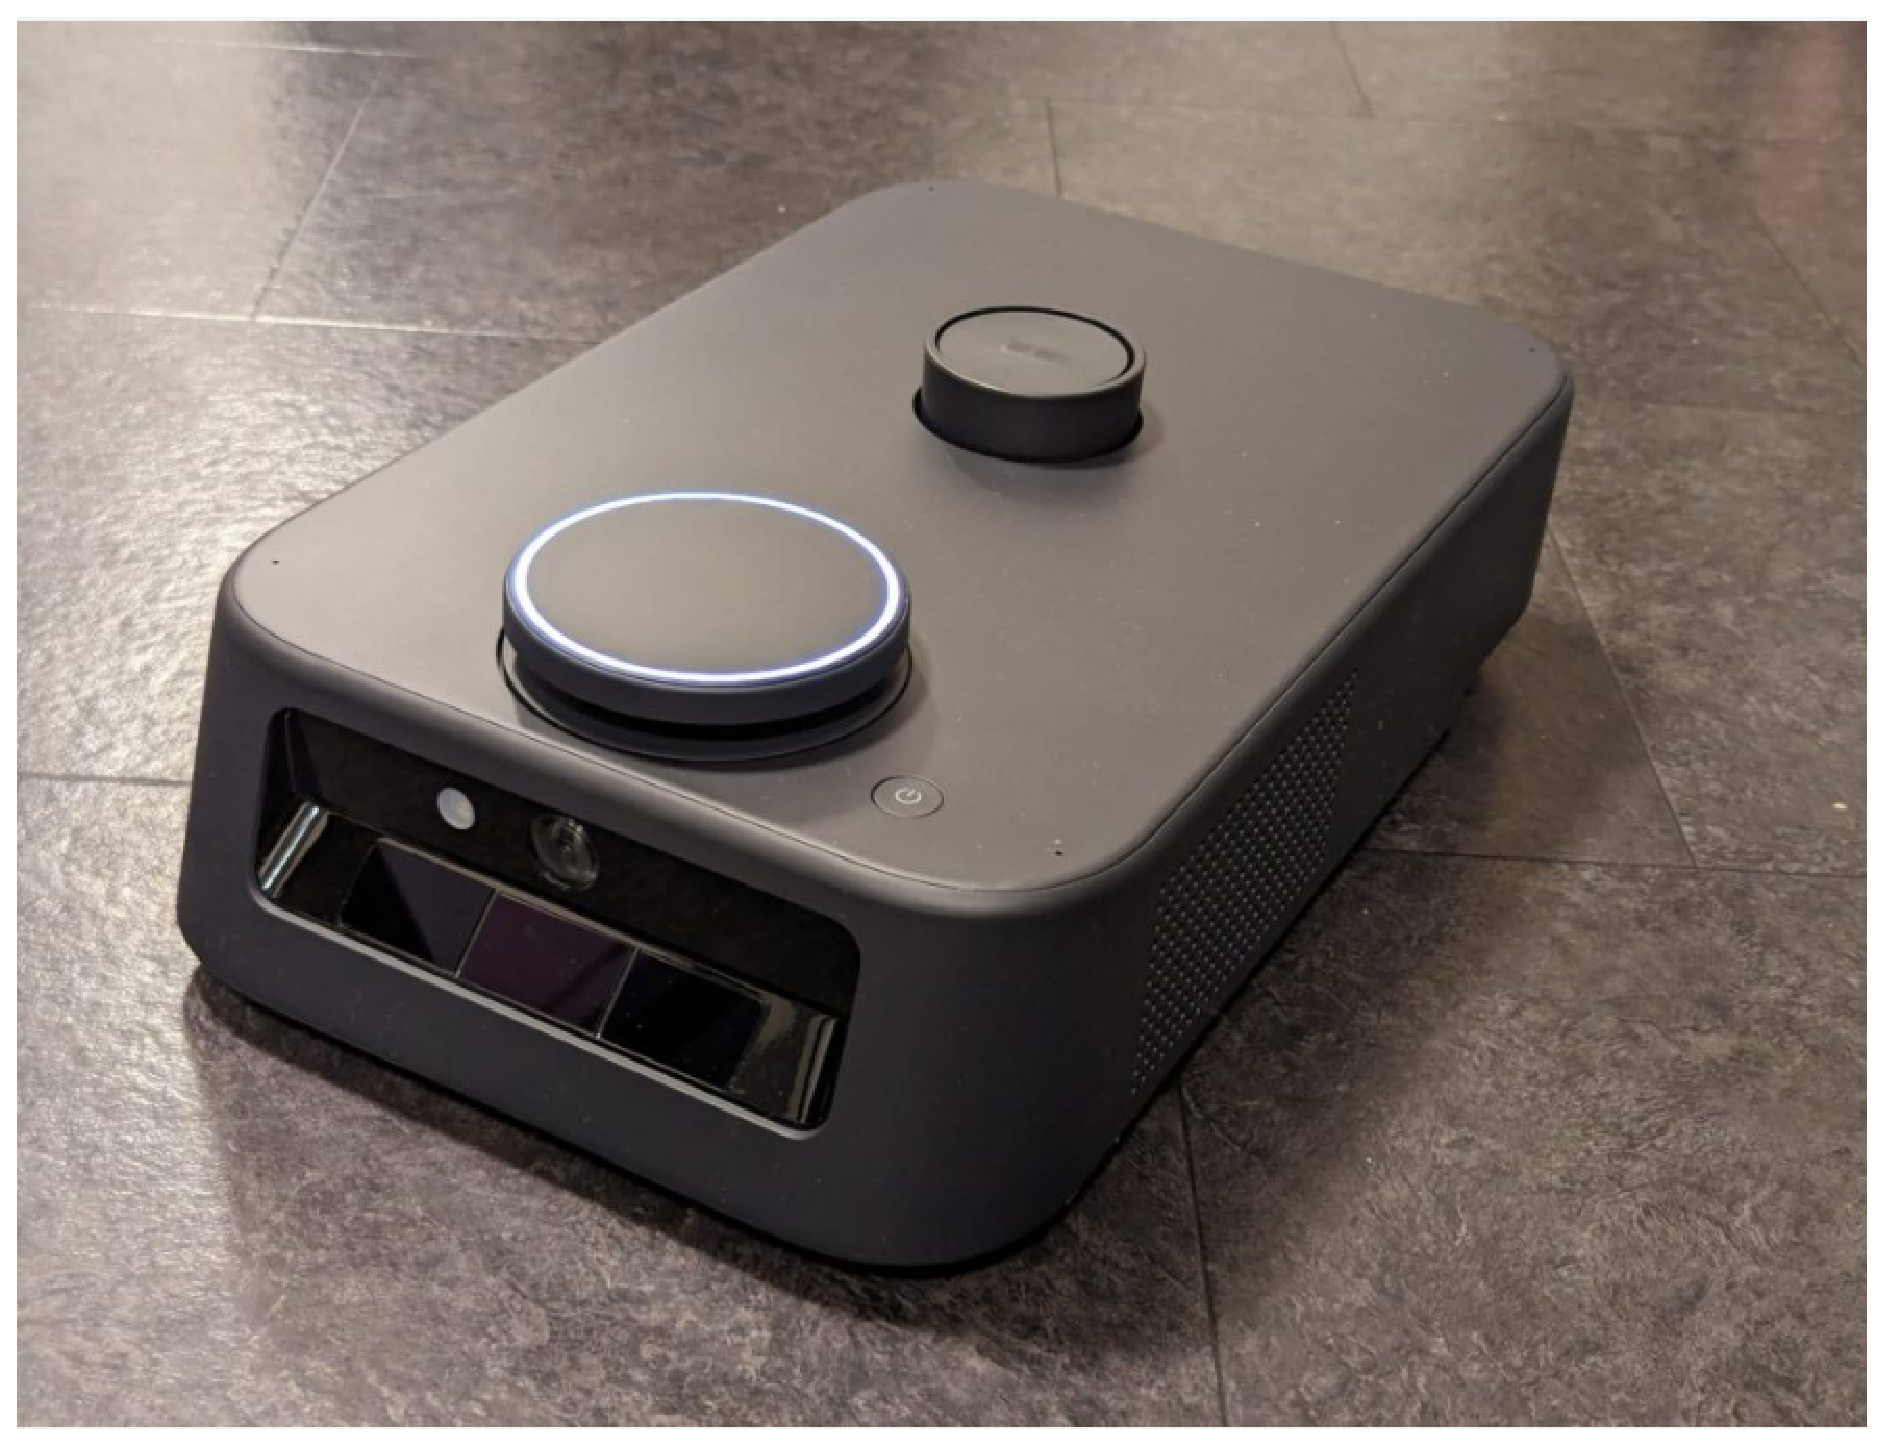
\includegraphics[height=30mm]{figure/kachaka.eps}
    \caption{カチャカ}
    \label{fig:kachaka}
  \end{minipage}
  \begin{minipage}[b]{0.45\linewidth}
    \centering
    \includegraphics[height=30mm]{figure/utm-30lx.eps}
    \caption{UTM-30LX}
    \label{fig:lidar}
  \end{minipage}
\end{figure}

\subsection{要求仕様}
本研究では, ロボット台車に株式会社Preferred Roboticsのカチャカを使用する. カチャカに北陽電機株式会社のUTM30-LXを搭載する. カチャカとUTM30-LXをそれぞれ図\ref{fig:kachaka}と図\ref{fig:lidar}に示す.制御PCは、NVIDIA GeForce GTX 1070 8GBを搭載しているノートPCを選定している.

以上の構成で以下の要求仕様を設定する.
\begin{enumerate}
    \item 2D-LiDARのデータで人追従ができる
    \item 雑多な環境下でも人追従ができる
    \item 0.8[m/s]以下の歩行速度で追従する
\end{enumerate}
\subsection{データセットの作成}
2D-LiDARのデータを俯瞰画像へ変換し, データセットを作成する. 2D-LiDARのデータは, ロボットが静止した状態で前方に人が2人ランダムに歩行する状態で, ROS2のBag機能で/scanトピックを保存した. ROS2 Bagのデータを元に12032枚の俯瞰画像を生成し, 人の両脚部をpersonクラスとしてアノテーションを行った. 図\ref{fig:dataset}にデータセットの例を示す. また, データ拡張を行うことにより, 10万枚のデータセットを作成する.
\subsection{YOLOv10による学習}
学習では, NVIDIA GeForce RTX 4090 24GBを搭載しているPCを使用し学習する. 過学習を抑制するため, Early Stoppingを設定する. また、学習時に使用する初期重みはYOLOv10-N, YOLOv10-S, YOLOv10-M, YOLOv10-B, YOLOv10-L, YOLOv10-Xを使用し、リアルタイム性と検出精度が最もバランスの良い重みをシステムに実装する.
\subsection{ロボット台車の制御}
YOLOv10による物体検出での推論結果から目標座標を生成し, ロボットから目標座標までの角度の偏差と距離の偏差を収束させるため, PD制御を実装する.

時刻$t$での, ロボットの座標から目標座標までの角度の偏差を$\theta(t)$とし, ロボット台車から取得できる旋回速度を$\omega(t)$とすると, ロボット台車の制御量である旋回速度$u(t)$以下のようになる.
\begin{equation}
\label{angularPD}
u(t) = K_p \theta(t) + K_d \left\{\frac{d}{dt} \theta(t) - \omega(t) \right\}
\end{equation}
$K_p$, $K_d$はそれぞれ比例ゲインと微分ゲインである. (\ref{angularPD})式の第1項は, ロボットの座標から目標座標までの角度の偏差を比例制御している. 第2項は, 実機での制御を考慮し, 不足しているまたは過多な制御量を微分制御により調整している.

%% 謝辞(必要な場合のみ)
%%\begin{acknowledgements}
%%\end{acknowledgements}

\section{実験}
\subsection{実験方法}
実験では, 要求仕様(2)を検証するため, 雑多な環境を作成し追従実験をする. 雑多な環境では, 人の脚部に類似している障害物を複数設置する. 人間は追従対象の1人と, 周囲を歩行する2〜3人を想定する. ここでは, 追従対象者とロボットの間を他の人間が通過することは想定しない. 実験する経路は, 直線経路, 曲線経路, 直角経路をそれぞれ10回実験する. 雑多な環境下における直線経路, 曲線経路, 直角経路をそれぞれ図\ref{fig:straight}, 図\ref{fig:curve}, 図\ref{fig:right-angle}に示す. また, 要求仕様(3)を検証するため, 雑多な環境下での10[m]以上の直線経路において, 提案するシステムが追従できる最大速度を検証する. 0.1[m/s]から0.1ずつ速度を上昇させ, 追従できなくなる速度の1つ前の速度を最大追従速度とする. これを, 最大追従速度実験とする. 要求仕様(2), (3)が満たされたら, 要求仕様(1)も満たされたものとする.
\subsection{考察}
期待される実験結果として, 雑多な環境下での直線経路における追従は可能であると考えられる. これは、経路の両端に雑多な環境を構築しており, 直線経路では両端に追従対象者が接近しないため, 追従対象者の脚部と脚部に類似した障害物を誤検出する可能性が低いためである.しかし、曲線経路と直角経路では追従が困難になると予想される. これは, 曲線経路と直角経路では, 人間が経路の両端に接近するため, 追従対象者の脚部と障害物を誤検出し, 追従対象者へは追従せず脚部に類似した障害物に追従し始めると考えられる.

\begin{figure}[tb]
  \centering
  \large
  % eps 画像を貼る場合は includegraphics をお使いください。
  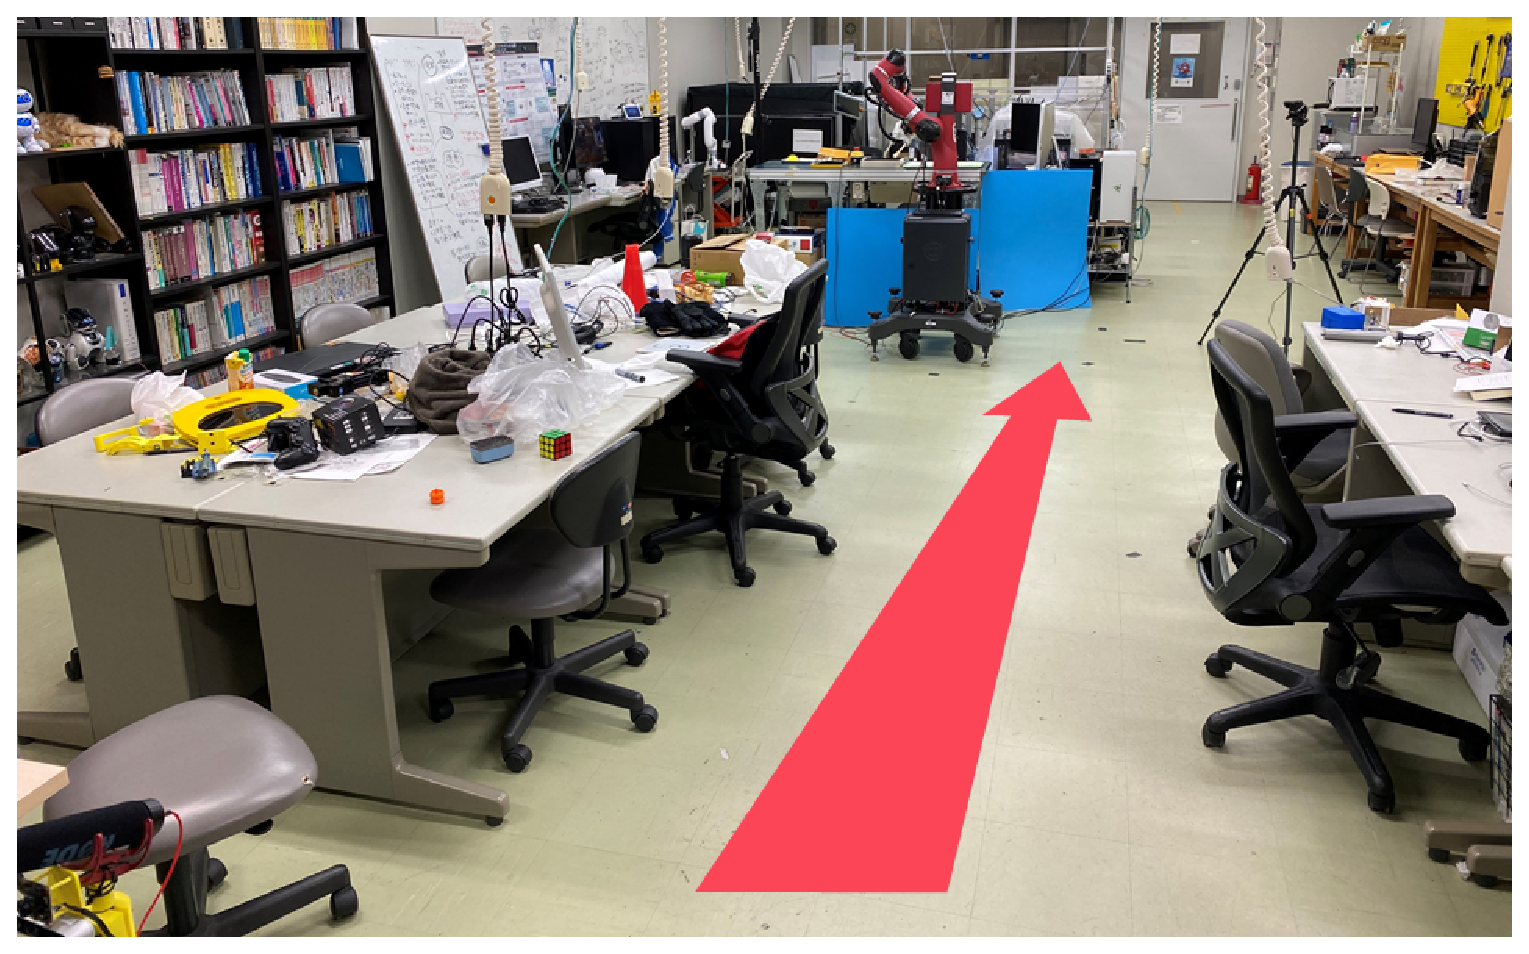
\includegraphics[width=55mm]{figure/straight.eps}
  \caption{直線経路のイメージ}
  \label{fig:straight}
\end{figure}

\begin{figure}[tb]
  \centering
  \large
  % eps 画像を貼る場合は includegraphics をお使いください。
  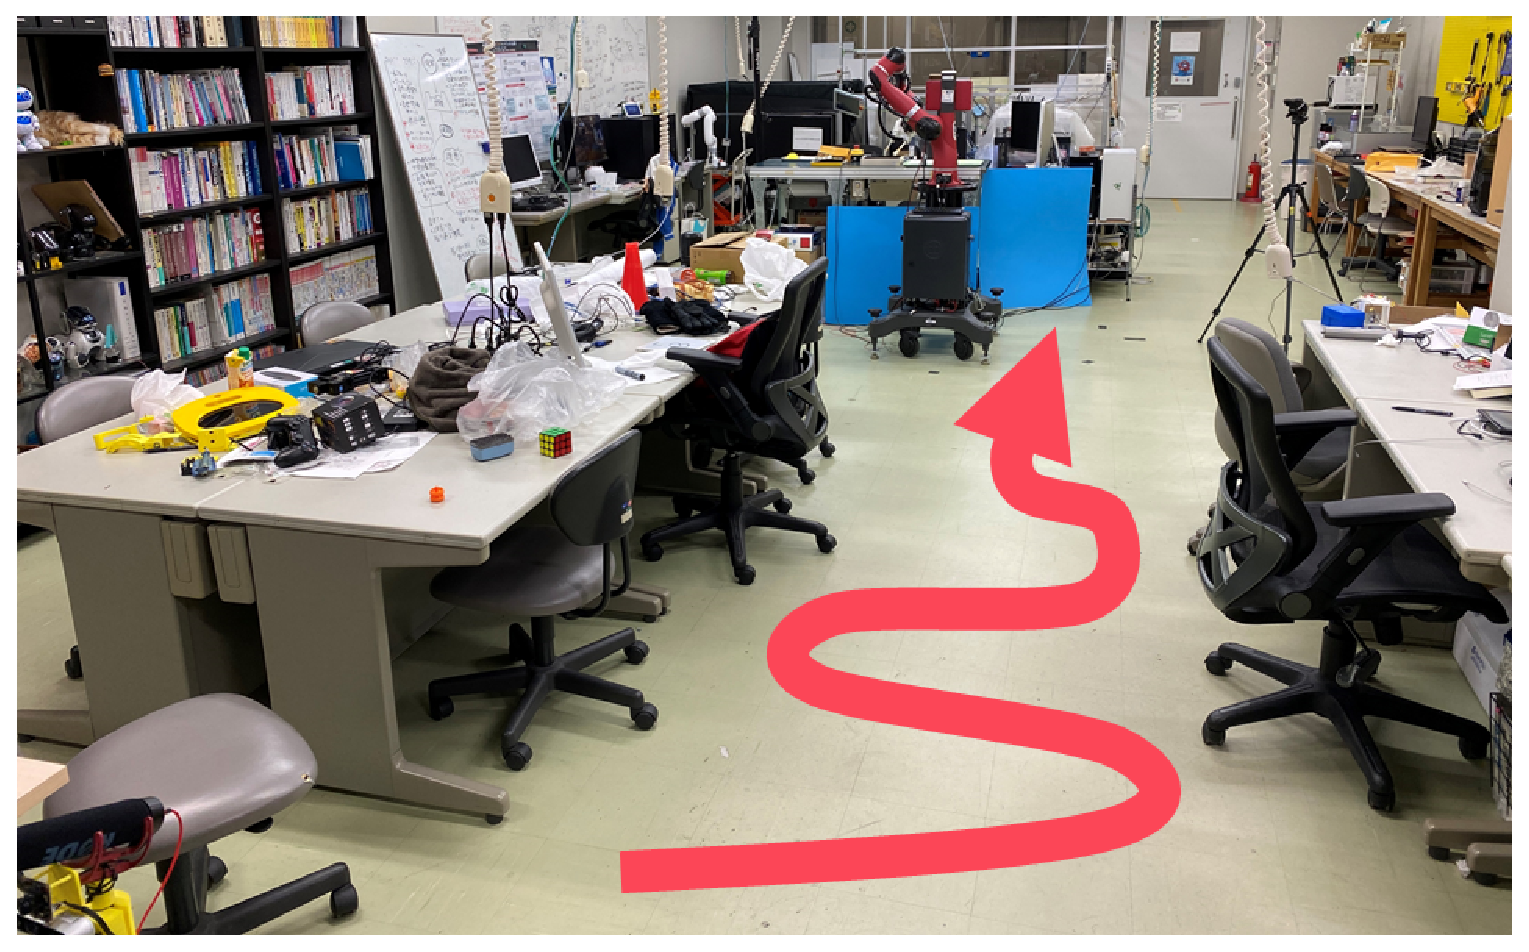
\includegraphics[width=55mm]{figure/curve.eps}
  \caption{曲線経路のイメージ}
  \label{fig:curve}
\end{figure}

\begin{figure}[tb]
  \centering
  \large
  % eps 画像を貼る場合は includegraphics をお使いください。
  \includegraphics[width=55mm]{figure/right-angle.eps}
  \caption{直角経路のイメージ}
  \label{fig:right-angle}
\end{figure}

\section{結言}
本研究では, 2D-LiDARの距離データとYOLOv10を用いた人追従システムの開発を行い, 雑多な環境下での追従実験と最大追従速度実験を行う予定である.

今後の課題として, 人の脚部と類似している障害物を誤検出し, 追従対象者への追従が途切れることが予想されるため, 雑多な環境下での追従精度を向上させる.



%% 謝辞(必要な場合のみ)
%\begin{acknowledgements}
%    Thanks.
%\end{acknowledgements}

\small
\begin{thebibliography}{9}
%%%%%%%%%%%%%%%%%%%%%%%%%%%%%%%%%%%%%%%%%%%%%%%%%%%%%%%%%%%%%%%%%%%%%%%%%%%%%%%

\bibitem{yolov10}
  Ao Wang, Hui Chen, Lihao Liu, Kai Chen, Zijia Lin, Jungong Han and Guiguang Ding: "YOLOv10: Real-Time End-to-End Object Detection", arXiv preprint arXiv:2405.14458,2024.
\bibitem{mahmudul2020}
  Mahmudul Hasan, Junichi Hanawa, Riku Goto, Hisato Fukuda, Yoshinori Kuno and Yoshinori Kobayashi: "Tracking People Using Ankle-Level 2D LiDAR for Gait Analysis", Advances in Artificial Intelligence, Software and Systems Engineering, pp.40-46, 2020.
\bibitem{angel2019}
  Angel Manuel Guerrero-Higueras, Claudia Álvarez-Aparicio, Mara Carmen Calvo Oliv-
era, Francisco J. Rodrguez-Lera, Camino Fernández-Llamas, Francisco Martn Rico and
Vicente Matellán, ”Tracking People in a Mobile Robot From 2D LIDAR Scans Using Full
Convolutional Neural Networks for Security in Cluttered Environments”, Frontiers in Neu-
rorobotics, Volume 12, Article 85, 2019.
%%%%%%%%%%%%%%%%%%%%%%%%%%%%%%%%%%%%%%%%%%%%%%%%%%%%%%%%%%%%%%%%%%%%%%%%%%%%%%%
\end{thebibliography}

\end{document}
